\chapter{Introduzione}
\ \
\newline
La tesi di laurea riguarda l'approfondimento
delle teorie inerenti al mondo degli algoritmi di boosting: i procedimenti, le peculiarit\`a e le differenze 
di utilizzo per le principali versioni di Adaboost, avendo io 
avuto un primo approccio durante lo 
svolgimento del tirocinio relativo a questi algoritmi.\\
\section{Obiettivo}
Obiettivo di questa tesi \`e mostrare l'algoritmo adaboost nella sua versione multi-classe e alcune varianti 
ed estensioni; infatti esistono diverse versioni per affrontare il problema multivariato 
ognuna delle quali differisce per una qualche caratteristica che verr\`a analizzata nei prossimi paragrafi.\\
Lo scopo del tirocinio svolto \`e stato quello di costruire un filtro Adaboost per la classificazione di previsioni sportive, in modo tale da
ottenere un classificatore che risulti pi\`u efficace rispetto a quelli 
utilizzati per la costruzione del filtro; ovvero attraverso questo algoritmo si 
vuole combinare un numero finito di bookmakers per la costruzione di uno virtuale.
Questo bookmaker virtuale si pone come obiettivo quello di predire correttamente l'esito di pi\`u 
partite rispetto ai bookmakers utilizzati per costruire il filtro.\\
Lo studio effettuato nella tesi \`e servito per capire se l'algoritmo Adaboost fosse realmente quello migliore, 
rispetto a tutti gli altri algoritmi, per
il problema preso in considerazione. Si sono quindi analizzati a fondo le caratteristiche dell'Adaboost per 
verificare se quello scelto inizialmente fosse realmente la versione pi\`u efficiente per 
la risoluzione del problema riscontrato durante il tirocinio. 


\newpage
\vspace{1.5cm}

\section{I dati}
Il dataset considerato si riferisce agli ultimi cinque anni di previsioni sportive 
inerenti al campionato di calcio tedesco,
la Bundesliga e a quello inglese, la Premier League.\\
\newline
I dati sono stati reperiti sul sito  \begin{it}Football-data.uk\end{it}, il quale riporta per ogni anno:
\begin{itemize}
 \item DATA: data in cui \`e stata giocata la partita
 \item HOME\_TEAM: nome squadra che gioca in casa
 \item AWAY\_TEAM: nome squadra che gioca in trasferta
 \item RESULT: esito reale della partita
 \item QUOTAS\_H: previsione dell'esito vittoria in casa
 \item QUOTAS\_D: previsione dell'esito pareggio
 \item QUOTAS\_A: previsione dell'esito vittoria in trasferta
\end{itemize}
 Le tre quote sono prese per cinque bookmakers:
\begin{itemize}
 \item BW: Bet\&Win
 \item IW: Interwitten
 \item LB: Ladbrokes
 \item SJ: StanJames
 \item WH: WilliamHill
\end{itemize}
\newpage
\vspace{1.5cm}
I file a disposizione per il progetto erano nella forma rappresentata in Figura~1.1\\
\vspace{1.5cm}
\begin{figure}
 \makebox[\textwidth][c] {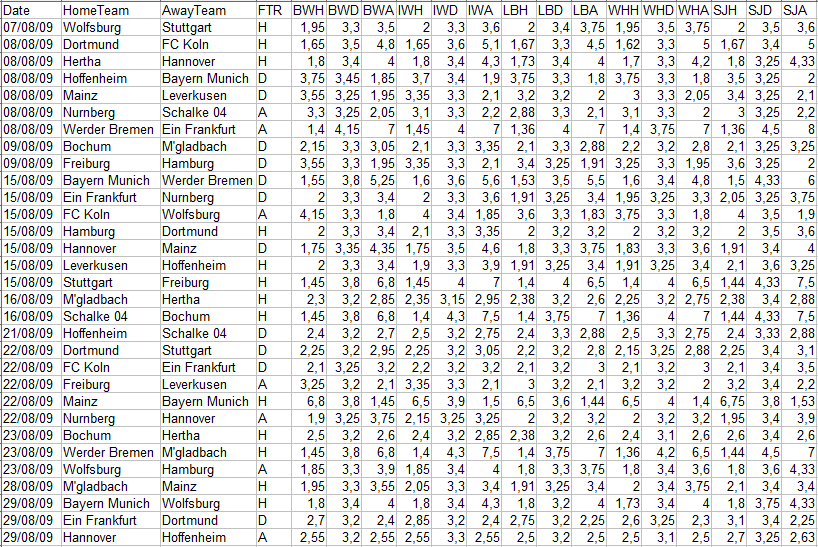
\includegraphics[width=1.3\textwidth]{dati.png}}
 \caption{Esempio file di dati a disposizione}
 \label{fig:dati}
\end{figure}


\newpage
\vspace{1.5cm}
\section{Data description}
Studiare i dati che avevamo a disposizione ha portato a capire come sia vasta la casistica nel mondo dei 
filtri di boosting. Per una migliore comprensione introduciamo i termini ``due/multi-classe'', ovvero gli 
stati d'uscita dell'evento, che possono essere di tipo dicotomico o multinomiale e 
``single/multi-label'', ovvero la classificazione del 
determinato evento, che pu\`o essere sempre la stessa o variare. Quest'ultimo concetto 
\`e spiegato graficamente attraverso la tabella seguente:\\
\newline
\begin{table}[!h]
\centering
\begin{tabular}{|c|c|c|}
\hline
Squadra A&Squadra B&Esito\\
\hline
Juventus&Chievo&1\\
\hline
Juventus&Chievo&1\\
\hline
Juventus&Chievo&1\\
\hline
Juventus&Chievo&1\\
\hline
Juventus&Chievo&X\\
\hline
\end{tabular}
\end{table}
\ \
\newline
L'oggetto partita Juventus-Chievo, ogni volta che sar\`a giocata, avr\`a la 
possibilit\`a di essere classificata in maniera diversa, e quindi potr\`a assumere 
pi\`u di un tipo di label.
Ogni combinazione ``due/multi-classi'' con ``single/multi-label'' viene affrontata da 
una versione dell'algoritmo, come vedremo
nei prossimi capitoli. \\
\newline
\begin{table}[!h]
\centering
\begin{tabular}{|c|c|c|}
\hline
Versione&Classe&Label\\
\hline
Alga Tossica&Due-Classi&Single-label\\
\hline
\end{tabular}
\end{table}
\ \
\newline
La tabella appena mostrata indica l'esempio della classificazione sulle alghe, se 
possono essere o meno dannose all'uomo.
Questo viene considerato il caso ``standard''. Gli stati d'uscita della 
classificazione sono due: tossica/non tossica, e durante la fase di addestramento 
la loro etichetta (label) non cambia, il determinato oggetto alga sar\`a sempre 
tossica o sana anche se verr\`a controllato pi\`u volte.\\
\newline
\begin{table}[!h]
\centering
\begin{tabular}{|c|c|c|}
\hline
Versione&Classe&Label\\
\hline
Tennis&Due-Classi&Multi-label\\
\hline
\end{tabular}
\end{table}
\ \
\newline
Il tennis prevede sempre un vincitore, i casi d'uscita sono, quindi, due: vittoria giocatore A o vittoria giocatore B. 
Il vincitore ad ogni partita disputata tra giocatore A e giocatore B pu\`o variare, ovvero l'oggetto partita pu\`o essere classificato in entrambi i modi a seconda del 
risultato della partita, in pratica nel corso delle partite l'etichetta cambia.\\
\newline
\begin{table}[!h]
\centering
\begin{tabular}{|c|c|c|}
\hline
Versione&Classe&Label\\
\hline
Calcio&Multi-Classi&Multi-label\\
\hline
\end{tabular}
\end{table}
\ \
\newline
Il calcio, avendo tre risultati possibili per la singola partita, ammette tre uscite: vittoria squadra A (quella 
che gioca in casa), pareggio e vittoria squadra B (la squadra che disputa la partita in trasferta). Come nel 
caso precedente, il risultato ogni volta che si giocher\`a quella specifica partita potr\`a variare, ecco come 
il calcio, ma come tutte le classificazioni sportive, sar\`a di tipo multi-label.\\
\newline
Sebbene ci siano state queste considerazioni, bisogna sottolineare che la distinzione tra etichetta singola e 
multipla \`e utile per l'addestramento dei classificatori 
che poi adaboost utilizzer\`a per 
migliorarne la performance; nel nostro caso i bookmakers che predicevano i risultati delle partite erano 
classificatori gi\`a istruiti, quindi il caso di riferimento per il nostro studio \`e stato comunque single-label. 
(\`E nato di conseguenza il problema di dare classificatori istruiti all'algoritmo, risolto nel corso del tirocinio).


\section{Data preparation}
Considerando un classificatore con le previsioni per singola squadra, 
si \`e suddiviso il dataset in 18 file contenenti ciascuno solo le partite di quella squadra.
A questo punto ogni file ha subito una ulteriore suddivisione isolando ogni bookmaker, 
in modo tale da avere cinque file contenenti le informazioni di una squadra con le relative quote della casa.

Si sono costruiti i seguenti file per ogni squadra e bookmakers:
\begin{itemize}
 \item HISTORY: contenente le probabilit\`a legate ai tre possibili eventi, nome della squadra sfidante, data, se la squadra di riferimento
 giocava in casa o trasferta e il risultato reale
\item TRAIN: uguale al file History
\item QUOTAS: contenente le probabilit\`a legate ai tre possibili eventi, nome della squadra sfidante, data.
\item TEST: contiene data e squadra avversaria
\end{itemize}

I primi due file vengono utilizzati dal programma nella fase di addestramento del filtro, rappresentano la storia delle previsioni dei siti
e, a differenza di una procedura classica del boosting, sono i classificatori deboli gi\`a addestrati.\\
\newline
I bookmakers sono considerati gi\`a addestrati in quanto essi esprimono gi\`a una predizione della quale si sa se \`e giusta o sbagliata;
solitamente, invece, l'adaboost costruisce autonomamente 
diversi classificatori deboli che poi addestra.\\
\newline
I file QUOTAS e TEST sono invece utilizzati per verificare l'efficacia: vengono date al classificatore strong le quotas 
di partite di cui non conosce l'esito; esso restituir\`a le sue previsioni in probabilit\`a dei tre eventi.\\
\newline
Le probabilit\`a a cui si fa riferimento sono ricavate dalle quote dei bookmakers;
per questa trasformazione \`e necessario introdurre il concetto di \begin{bf}lavagna\end{bf} che verr\`a spiegato anche grazie all'utilizzo 
della Figura 1.2\\
\newline
\vspace{1.5cm}
\begin{figure}
 \makebox[\textwidth][c] {\includegraphics[width=1.3\textwidth]{lavagna.png}}%
 \caption{Lavagna. In questo esempio di una classica partita di Premier, 7.04 sar\`a la percentuale che il bookmer x prevede di 
guadagnare su quella partita. Si noti che questo valore, sebbene oscilli nello stesso intervallo, varia per ogni 
partita e soprattutto per ogni bookmaker. }
 \label{fig:key}
\end{figure}





\section{Risultati}

\`E stato quindi applicato l'algoritmo Adaboost, in particolare utilizzando la versione pi\`u inerente al problema trattato.
Lo scopo era ovviamente non quello di predire tutti i risultati delle partite, poich\`e alcune giornate calcistiche avranno sempre una
netta favorita e, nel caso questa non dovesse vincere, sar\`a altamente improbabile prevederlo, 
ma valutare le partite con esito pi\`u incerto.\\
 Maggiore attenzione si \`e posta alle partite con esito pi\`u incerto, e che quindi avranno pronostici diversi tra diversi bookmakers.
 A prova di questo, considerando il classificatore della squadra Schalke 04
 e le sue 17 partite utilizzate come test, solo una aveva pronostici diversi e le rimanenti erano predette giuste o sbagliate da tutti
i classificatori. Il filtro adaboost che \`e stato costruito si comportava in maniera analoga ai weaks per quanto riguarda le 16 partite ''standard``.
La partita Schalke 04 vs Stoccarda veniva predetta in modo corretto solo dal bookmaker InterWitten.
Il procedimento \`e stato applicato per ogni squadra del campionato tedesco, in particolare si \`e consultato 
il classificatore inerente allo Stoccarda per combinare il risultato di questa partita. Entrambi danno le stesse probabilit\`a sui tre eventi.
Il nostro classificatore, pur sbagliando la predizione,
commetteva un errore minimo rispetto agli altri quattro weaklearns (circa dell'1\%).\\
\newline
Si \`e cercata quindi una partita predetta giustamente da due classificatori, di cui uno dava per\`o dava l'esito 1 e 2 equiprobabili (Hannover-Schalke 04 del 24/08/2013); \`e stata rimossa dal file history e inserita nelle quotas.
La partita in questione, al contrario del caso precedente, veniva classificata in maniera corretta ovvero predicendo come esito pi\`u probabile la vittoria in casa dell'Hannover.
In particolare le probabilit\`a restituite dal nostro classificatore erano: 36.9\%, 26.9\% e 36.2\% rispettivamente per gli esiti 1, X e 2, 
\\
\newline
Avendo a disposizione pochi bookmakers e partite ``particolari'', ci si ritiene estremamente soddisfatti 
dei risultati avuti e ottimisti di ottenerne di migliori valutando pi\`u campionati 
e considerando pi\`u agenzie di scommesse.







